\documentclass{beamer}
\mode<presentation>
% {
%   \usetheme{lankton-keynote}% oder CambridgeUS Darmstadt Singapore
%   \setbeamercovered{transparent}
% }
\usetheme{CambridgeUS} %Darmstadt
%\usetheme{Warsaw} %Darmstadt
\usepackage{color}
\usepackage[utf8]{inputenc}
\usepackage[german]{babel}
\usepackage{times}

\usepackage{graphicx}
\usepackage{multimedia}
\usefonttheme{serif}
%\usepackage{floatflt}
%\usepackage{float}
\usepackage{listings}
\definecolor{green}{rgb}{0,.5,0}  
\definecolor{darkblue}{rgb}{0,0,.6}
\definecolor{darkred}{rgb}{.6,0,0}
\definecolor{darkgreen}{rgb}{0,.6,0}
\definecolor{red}{rgb}{.98,0,0}
\definecolor{lightblue}{rgb}{0.8,0.85,1}

%silvio anfang
\definecolor{dunkelrot}{rgb}{0.4,0.0,0.0}
\definecolor{dunkelgreen}{rgb}{0.0,0.4,0.0}
\definecolor{blue}{rgb}{0.6,0.6,0.7}
\definecolor{black}{rgb}{0.01,0.01,0.01}
\definecolor{grau}{rgb}{0.2,0.2,0.2}
\definecolor{white}{rgb}{1.0,1.0,1.0}
\definecolor{blocktitle}{rgb}{0.2, 1.0, 0.1}
\definecolor{blockbody}{rgb}{0.9, 0.9, 0.9}
\definecolor{ablocktitle}{rgb}{0.6, 0.1, 0.1}
\definecolor{ablockbody}{rgb}{0.9, 0.9, 0.9}
\definecolor{eblocktitle}{rgb}{0.1, 0.5, 0.1}
\definecolor{eblockbody}{rgb}{0.9, 1.0, 0.9}
\definecolor{itemfront}{rgb}{0.7, 0.2, 0.2}
\definecolor{itemback}{rgb}{0.0, 0.0, 0.0}
\setbeamercolor{palette primary}{use=structure,fg=dunkelrot,bg=blue}%ueberschrift schrift, ueberschrift hintergrund 
%\setbeamercolor{palette secondary}{use=structure,fg=black,bg=dunkelgreen}%??, frametitle rechts
%\setbeamercolor{palette tertiary}{use=structure,fg=black,bg=magenta}%ohne
\setbeamercolor{palette quaternary}{use=structure,fg=dunkelgreen,bg=black}%schrift headline+framtitle, hintergrund headline + framtitle links
\setbeamercolor{title}{bg=blockbody}
\setbeamercolor*{block title}{bg=blocktitle}
\setbeamercolor*{block body}{bg=blockbody}
\setbeamercolor*{block title alerted}{bg=ablocktitle}
\setbeamercolor*{block body alerted}{bg=ablockbody}
\setbeamercolor*{block title example}{bg=eblocktitle}
\setbeamercolor*{block body example}{bg=eblockbody}
\setbeamercolor*{item}{bg=itemback}
\setbeamercolor*{item}{fg=itemfront}
\setbeamerfont{frametitle}{size=\large}
\setbeamerfont{normal text}{size=\small}
%silvio ende

\lstloadlanguages{SQL}
\lstset{%
  language=SQL,
  basicstyle=\footnotesize\ttfamily,
  commentstyle=\itshape\color{darkgreen},
  keywordstyle=\bfseries\color{darkblue},
  stringstyle=\color{darkred},
  showstringspaces=false,
  breaklines=true
}%

\setbeamersize{text margin left=5mm}

\AtBeginSection[]
{
  \begin{frame}<beamer>{}
    \tableofcontents[currentsection,currentsubsection,hideothersections,hideothersubsections]
  \end{frame}
}

\title[Vergleich von SQL-Anfragen]{Vergleich von SQL-Anfragen:\\Theorie und Implementierung in Java}

%\subtitle{sub} % ()

\author[Robert Hartmann]{Robert Hartmann}

\institute[] % (optional)
{
  Martin-Luther-Universität Halle-Wittenberg\\
  Naturwissenschaftliche Fakultät III\\
  Institut für Informatik
}

\date[]{26. September 2013}

\subject{Informatik}


\begin{document}

\begin{frame}
  \titlepage
\end{frame}

\begin{frame}{}
  \tableofcontents
\end{frame}

\section{Einleitung}
\subsection{Motivation}

\begin{frame}{Motivation}
\begin{itemize}
\item Vergleich von SQL-Anfragen üblicherweise in der Lehre
\item Übungsaufgaben notwendig für praktisches Verständnis von SQL
\item Bestehend aus Sachaufgabe und Datenbankschema
\item Lösung des Lernenden formuliert als SQL-Statement
\end{itemize}
\pause
\begin{alertblock}{semantische Äquivalenz}
Zwei SQL-Anfragen sind semantisch äquivalent, wenn beide Anfragen auf allen Datenbankzuständen einer Datenbank stets die selben Tupel zurückliefern.
\end{alertblock}

\begin{itemize}
\item Allgemein: Nicht entscheidbar
\item Korrektur der Aufgabe auf zwei Arten: manuell oder automatisch
\end{itemize}

\end{frame}

\begin{frame}{Manueller Vergleich}
\begin{block}{Vorteile}
\begin{itemize}
\item Korrektur zuverlässig 
\item Syntaktische Varianten der Lösung werden erkannt
\item Lernender erhält (potentiell) detailliertes Feedback
\end{itemize}
\end{block}

\begin{alertblock}{Nachteile}
\begin{itemize}
\item Korrektur langsam
\item Wenig Geld und Kürzungen in Lehre $\to$ Wenig Zeit zur Verfügung
\item Unter Zeitdruck: Mehr Fehler, wenig detailliertes Feedback
\end{itemize}
\end{alertblock}

\textbf{Fazit}: Manuelles Vergleichen funktioniert nur, wenn genug Mitarbeiter/ Hilfskräfte zur Verfügung stehen.
\end{frame}

\begin{frame}{Automatischer Vergleich}
Automatischer Vergleich zweier SQL-Anfragen wird üblicherweise durch den Vergleich der Ergebnistupel realisiert.
\begin{block}{Vorteile}
\begin{itemize}
\item Korrektur in Echtzeit
\item Keine Mitarbeiter oder Hilfskräfte benötigt
\end{itemize}
\end{block}

\begin{alertblock}{Nachteile}
\begin{itemize}
\item Für jedes Datenbankschema sind Daten notwendig
\item Feedback für Lernenden oft unzureichend um Fehler zu identifizieren
\item \textit{false positive} leicht zu erstellen, System kann ausgehebelt werden
\item \textit{false positive} auch unabsichtlich problematisch: Lernender bemerkt Fehler nicht
\end{itemize}
\end{alertblock}

\textbf{Fazit}: Automatisches Vergleichen durch bloßes Vergleichen von Ergebnistupeln nicht zuverlässig
\end{frame}

\subsection{Überblick des neuen Ansatzes}

\begin{frame}{Neuer Ansatz}
\begin{itemize}
\item automatischer Vergleich mit Datenbankschema und Musterlösung
\item sichere Rückmeldung benötigt Daten, Hauptteil aber ohne möglich
\end{itemize}
\pause
Erster Schritt: \textbf{Standardisierung} (Prüfung: hinreichende Bedingung) \\
\textbf{Ziel}: Semantisch äquivalente Anfragen sollen nach der Standardisierung auch syntaktisch gleich sein \\
\vspace{4mm}\pause
Zweiter Schritt: \textbf{Vergleich von Ergebnismengen} (Prüfung: notwendige Bedingung)\\
\textbf{Ziel}: Nachweis der Ungleichheit beider Anfragen \\
\vspace{4mm}\pause
Dritter Schritt: \textbf{Struktureller Vergleich der Anfragen}\\
\textbf{Ziel}: genauere Lokalisierung von Fehlern des Lernenden
\end{frame}


\section{Standardisierung}

\begin{frame}[fragile]{Überblick}
\begin{itemize}
\item Standardisierung bildet ersten Schritt 
\item Entfernen von syntaktischen Details und Einlesen von Anfrage in Datenstruktur durch Parser
\item Behandeln von einzelnen Teilen der SQL-Anfrage (\verb|SELECT, FROM, WHERE, GROUP BY, ORDER BY|)
\item Abarbeitung nicht streng hintereinander, da einige Teile abhängig sind
\item Zusammensetzen der behandelten Teile zur standardisierten SQL-Anfrage
\end{itemize}
\end{frame}




%subsection einzelne teile 

\begin{frame}[fragile]{FROM-Teil}
\begin{itemize}
\item Lexikographisches Sortieren der Tabellen
\item Einführung künstlicher Tupelvariablen (TV) mit fortlaufender Nummerierung (a1,a2,...)
\item TV auf gleicher Ebene erhalten gleichen Startwert für Iteration
\end{itemize}
\pause
\begin{verbatim}
SELECT ename FROM emp
WHERE sal > (SELECT AVG(sal) FROM emp)
AND empno > (SELECT AVG(empno) FROM emp)
\end{verbatim}
\pause
\begin{verbatim}
SELECT ename FROM emp a1
WHERE sal > (SELECT AVG(sal) FROM emp a2)
AND empno > (SELECT AVG(empno) FROM emp a2)
\end{verbatim}
\end{frame}

\begin{frame}[fragile]{SELECT-Teil}
\begin{itemize}
\item Ersetzen von Wildcard (*) zu konkreten Spalten (vor Sortieren in \verb|FROM|)
\item Einführen der künstlichen TV als Aliase
\item Wenn Spaltenreihenfolge unwichtig: lexikographisches Sortieren der Spalten
\end{itemize}
\pause
\begin{verbatim}
SELECT ename FROM emp a1
WHERE sal > (SELECT AVG(sal) FROM emp a2)
AND empno > (SELECT AVG(empno) FROM emp a2)
\end{verbatim}
\pause
\begin{verbatim}
SELECT a1.ename FROM emp a1
WHERE a1.sal > (SELECT AVG(a2.sal) FROM emp a2)
AND a1.empno > (SELECT AVG(a2.empno) FROM emp a2)
\end{verbatim}
\end{frame}


\begin{frame}[fragile]{WHERE-Teil - syntaktische Varianten}
\begin{itemize}
\item Umwandeln des \verb|WHERE|-Ausdrucks in KNF (konjunktive Normalform) 
\item[$\to$] Erhöhung der Lesbarkeit, Eliminierung von unnötig tiefen Teilbäumen
\end{itemize}
Entfernung von syntaktischen Varianten:\pause
\begin{itemize}
\item \verb|a BETWEEN l AND u| zu \verb|a >= l AND a <= u|
\item \verb|a >= ALL(c1, c2, c3)| zu \verb|a >= c1 AND a >= c2 AND a >= c2|
\item \verb|a >= ANY(c1, c2, c3)| zu \verb|a >= c1 OR a >= c2 OR a >= c2|
\item \verb|EXISTS (SELECT expr FROM ...)| zu \verb|EXISTS (SELECT 1 FROM ...)|
\end{itemize}
\end{frame}

\begin{frame}[fragile]{WHERE-Teil - Arten von Operatoren}
\begin{itemize}
\item \verb|WHERE|-Ausdruck besteht im wesentlichen aus Operatoren, Konstanten und Spaltennamen
\item Ordnung wird benötigt, damit semantisch äquivalente Anfragen auch syntaktisch gleich sind
\end{itemize}\pause
\textbf{Arten von Operatoren:}
\begin{itemize}
\item Operatoren: \verb|IS NULL, IS NOT NULL, EXISTS, ANY/SOME, ALL, ...|
\item[$\to$] keine syntaktischen Varianten möglich
\item nicht-kommutative Operatoren: $\leq,\geq,<,>,-,/$
\item[$\to$] Hinzufügen aller Schreibweisen
\item kommutative Operatoren: $=,<>,+,*,AND,OR$
\item[$\to$] Alle Permutationen der Operanden sind gültig $\to$ Festlegung einer Ordnung
\end{itemize}

\end{frame}



%\begin{frame}[fragile]{WHERE-Teil - Operatorenvielfalt (1)}
%\textbf{Problem:} Ausdrücke können unterschiedlich aufgeschrieben werden. Es ist nicht klar, welche Schreibweise der Lernende verwenden wird.\\
%\textbf{Beispiel:} \verb|a > 3| äquivalent zu \verb|3 < a| und mit Zusatzwissen auch zu \verb|a >= 2| und \verb|2 <= a|\\
%\vspace{5mm}
%\textbf{Ansatz 1:} Hinzufügen aller äquivalenten Ausdrücke\\
%\textbf{Ansatz 2:} Zulassen einer Repräsentation und Verbieten der restlichen Schreibweisen\\
%\vspace{5mm}
%Wir verfolgen den implementierten Ansatz 1.
%\end{frame}





\begin{frame}[fragile]{Ordnung bei kommutativen Op}
\begin{itemize}
\item Baum $T(x)$ mit Wurzel $x$. $children(x) = (c_1,c_2,...,c_n)$
\item Reihenfolge von $children(x)$ beliebig veränderbar
\item[$\to$] Eindeutige Repräsentation erfordert Ordnung von $children(x)$\pause
\item $order: children \to \mathbb{N}$
\item Nach Sortieren gilt: $order(c_1) \leq order(c_2) \leq ... order(c_n)$
\end{itemize}
\begin{tabular}{|l|l|l|l|l|l|l|l|l|l|l|l|l|l|l|l|}
\hline
$r$ & Spalte & Konstante & OR & $\le$ & $\ge$ & $<$ & $>$ & $=$ & $<>$ & $+$ & ...\\\hline
$\textit{order}(r)$ & 1 & 2 & 3 & 4 & 5 & 6 & 7 & 8 & 9 & 10 & 11\\ 
\hline
\end{tabular}\newline
%\begin{tabular}{|l|l|l|l|l|l|l|l|l|l|l|l|l|l|l|l|}
%\hline
%$r$  & $/$  & IS NULL & IS NOT NULL & EXISTS & ANY & ALL & NOT \\\hline
%$\textit{order}(r)$ &   12 & 13& 14 & 15 & 16 & 17  & 18\\ 
%\hline
%\end{tabular}
\vspace{3mm}
\begin{itemize}
\item Vorgehen: BOTTOM-UP durch Rekursion
\end{itemize}
\end{frame}

\begin{frame}[fragile]{WHERE-Teil - Sortierung (2)}
Beispiel:\\
\verb|d = 5 OR a < 6| $\ \ \to\ \ $ \verb|a < 6 OR d = 5|\\
\begin{center}
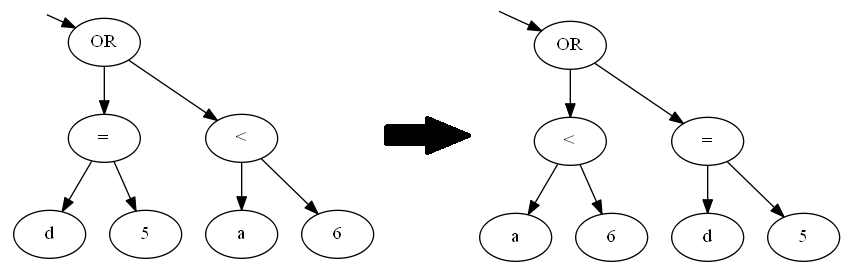
\includegraphics[scale=0.3]{sort_step1.png}
\end{center}\pause
\textbf{Problem: }Was passiert, wenn zwei Kinder den gleichen Operator bezeichnen oder beide Kinder Spaltennamen bzw. Konstanten sind?
\end{frame}

\begin{frame}[fragile]{Beide Kindknoten bezeichnen gleichen Operator}
\visible<2->{
\begin{itemize}
\item Situation: $order(c_i) = order(c_j)$ und $c_i,c_j$ sind Operatoren ($j = i + 1$)
\item[$\to$] Schrittweise Tiefensuche auf $T(c_i), T(c_j)\ \ $ Aktuelle Knoten in DFS: $v_i,v_j$
\item Wenn $v_i \neq v_j$ dann muss gelten: $order(v_i) < order(v_j)$, sonst Tauschen von $c_i,c_j$
\end{itemize}}
\textbf{Beispiel}:\\

\verb|b = 2 OR c IS NULL and a < 6 OR d = 5 AND a > 5|
\begin{center}
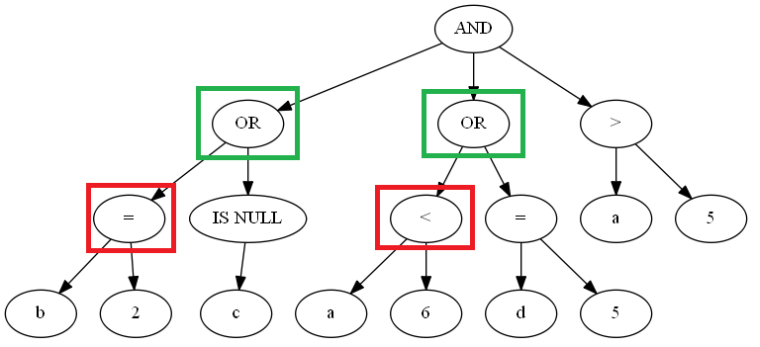
\includegraphics[scale=0.27]{sort_step2.png}
\end{center}

$\to$ Tauschen, da $order(=) = 8 > 6 = order(<) $\\
\end{frame}

%\begin{frame}[fragile]{Beide Kindknoten bezeichnen Spaltennamen/Konstanten}
%\begin{itemize}
%\item Situation: $order(c_i) = order(c_j)$ und $c_i,c_j$ sind Spaltennamen oder Konstanten mit ($j = i + 1$)
%\item[$\to$] lexikographische Sortierung
%\end{itemize}
%\textbf{Beispiel}:\\
%
%\verb|empno = deptno| wird zu \verb|deptno = empno|\\
%\vspace{4mm}
%\textbf{Abschließend:}
%\begin{itemize}
%\item Wiederherstellen der KNF 
%\item Entfernung von Duplikaten 
%\end{itemize}
%\end{frame}

%\begin{frame}[fragile]
%Es sei $T(x)$ ein Parserbaum mit $children(x) = (c_1,c_2,...,c_n)$. Haben wir $order(c_i) = order(c_{i+1})$ %benötigen wir weiteres Kriterium für Bestimmung eindeutiger Ordnung.
%Wir benutzen schrittweise Tiefensuche, da alle Bäume unter $c_i$ und $c_j$ bereits sortiert sind.
%\begin{itemize}
%\item Es sei $order(c_i) = order(c_j)$ mit $j = i + 1$ und $c_i,c_j$ sind beides keine Konstanten oder Variablen
%\item $DFS_i(x)$ bezeichnet aktuellen Knoten bei Tiefensuche auf Wurzelknoten $x$ im Schritt $i$.
%\item \begin{lstlisting}[mathescape]
%for k=1 to n
%   if ($DFS_k(c_j)$ == NULL) AND ($DFS_k(c_i)$ != NULL)
%   	  swap(c_j,c_i);
%   else if $order(DFS_k(c_j)) < order(DFS_k(c_i))$
%      swap(c_j,c_i);
%      return;
%   endif
%endfor
   
%\end{lstlisting}
%\end{itemize}
%\end{frame}


%\begin{frame}[fragile]{WHERE-Teil - Sortierung (4)}
%Gilt $order(c_i) = order(c_j)$ mit $j = i + 1$ und $c_i,c_j$ sind beides Konstanten oder Variablen, dann %entscheidet lexikographische Sortierung.\\
%\vspace{5mm}
%\textbf{Beispiel}:\\
%
%\verb|b = 2 OR c IS NULL and a < 6 OR d = 5 AND a > 5|
%\begin{center}
%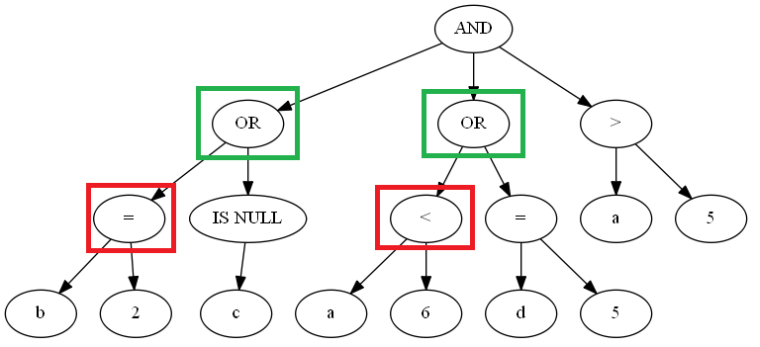
\includegraphics[scale=0.27]{sort_step2.png}
%\end{center}
%
%$\to$ Tauschen, da $order(=) = 8 > 6 = order(<) $\\
%\textbf{Letzter Schritt der Sortierung}: Entfernung von Duplikaten.
%\end{frame}



\begin{frame}[fragile]{Verbunde und Unterabfragen}
\begin{itemize}
\item Äußere Verbunde ersetzt durch inneren Verbund verknüpft mit \verb|UNION ALL|
\item Natürliche Verbunde unter \verb|FROM| als innere Verbunde unter \verb|WHERE|
\item Entfernen von Schlüsselwort \verb|CROSS JOIN|
\item Innere Verbunde unter \verb|FROM| werden unter \verb|WHERE| formuliert
\item Umwandeln sämtlicher Unterabfragen zu \verb|EXISTS|-Unterabfragen 
\end{itemize}
\end{frame}

\section{Vergleich mit realen Daten}



\begin{frame}[fragile]{Idee}
\begin{itemize}
\item iterativer Vergleich beider Ergebnismengen nicht ohne weiteres möglich
\item Problem: Optimierer des DBMS übernimmt Sortierung, wenn nicht explizit angegeben
\item selbst mit expliziter Angabe: Sortierung nicht notwendigerweise eindeutig
\item Beispiel: \\\verb|SELECT surname, firstname|\\\verb|FROM people ORDER BY surname|
\end{itemize}
\textbf{Probleme}:\pause\\
\begin{itemize}
\item Falsche Lösung wird zufällig korrekt sortiert $\to$ falsche Übereinstimmung
\item Korrekte Lösung wird falsch sortiert $\to$ keine Übereinstimmung 
\end{itemize}
\end{frame}


\begin{frame}[fragile]{Fallunterscheidung (1)}
\begin{itemize}
\item ML enthält kein \verb|ORDER BY| $\to$ \verb|ORDER BY| von LL streichen
\item künstliche Sortierung nach Auswahlspalten, die unbenutzt sind
\item iteratives Vorgehen
\end{itemize}
\textbf{Beispiel:}\\
\begin{verbatim}
SELECT firstname, surname, birthdate FROM people 
ORDER BY surname
\end{verbatim}\pause
zu:
\begin{verbatim}
SELECT firstname, surname, birthdate FROM people 
ORDER BY surname, 1, 3
\end{verbatim}
\begin{itemize}
\item[$\to$] SQL-Anfrage nun auf jedem DBMS immer eindeutige Ausgabereihenfolge
\end{itemize}
\end{frame}
%\begin{frame}[fragile]{Fallunterscheidung (1)}
%ML enthält kein \verb|ORDER BY|, LL enthält \verb|ORDER BY|
%\begin{itemize}
%\item Sortierung offensichtlich egal $\to$ zunächst Entfernung von \verb|ORDER BY| von LL
%\end{itemize}
%
%ML enthält ein \verb|ORDER BY|, LL enthält kein \verb|ORDER BY|
%\begin{itemize}
%\item Sortierung von Bedeutung
%\item Lernende ist Sortierung offensichtlich egal
%\item Ziel: Nachweisen der Ungleichheit $\to$ keine Anpassungen
%\item Problem: zufällige Übereinstimmung
%\end{itemize}
%
%ML enthält kein \verb|ORDER BY|, LL enthält \verb|ORDER BY|
%\begin{itemize}
%\item keine Anpassung
%\item Problem: zufällige Übereinstimmung
%\end{itemize}
%\end{frame}


\section{Hinweismeldungen}

\begin{frame}[fragile]{Feedback}
\begin{itemize}
\item Vergleich einzelner Teile der Anfrage (\verb|SELECT, FROM, ...|)
\item[$\to$] Hinweis an Nutzer, welche Teile identisch mit ML sind (WO ist der Fehler?)
\item Vergleich von Anzahl verschiedener Komponenten (Tabellen, Formeln, Verbunde, Unterabfragen)
\item[$\to$] konkreter Hinweis, WAS an der eigenen Lösung fehlt/überflüssig ist
\item Vergleich mit Realdaten (Schritt 2) unterstützt verschiedene DBMS $\to$ verschiedene Fehlermeldung der DBMS beim Parsen mit DBMS-Parser
\item[$\to$] Kompatibilitätstest 
\end{itemize}
\end{frame}


\section{Implementierung}


\begin{frame}[fragile]{Technische Details}
Ergebnisse der Arbeit sollen in Form einer Lernplattform umgesetzt werden.
\vspace{5mm}
\begin{itemize}
\item Javaklassen per JSP als HTML-Seiten nutzbar
\item[$\to$] plattformunabhängig
\item automatisches Build- und Deployskript per \textit{ant}
\item Parser: ZQL (Open Source)
\item mögliche DBMS für Schritt 2: alle mit JDBC-Connector 
\end{itemize}
\end{frame}

\begin{frame}[fragile]{Aufbau des Programms}
\begin{center}
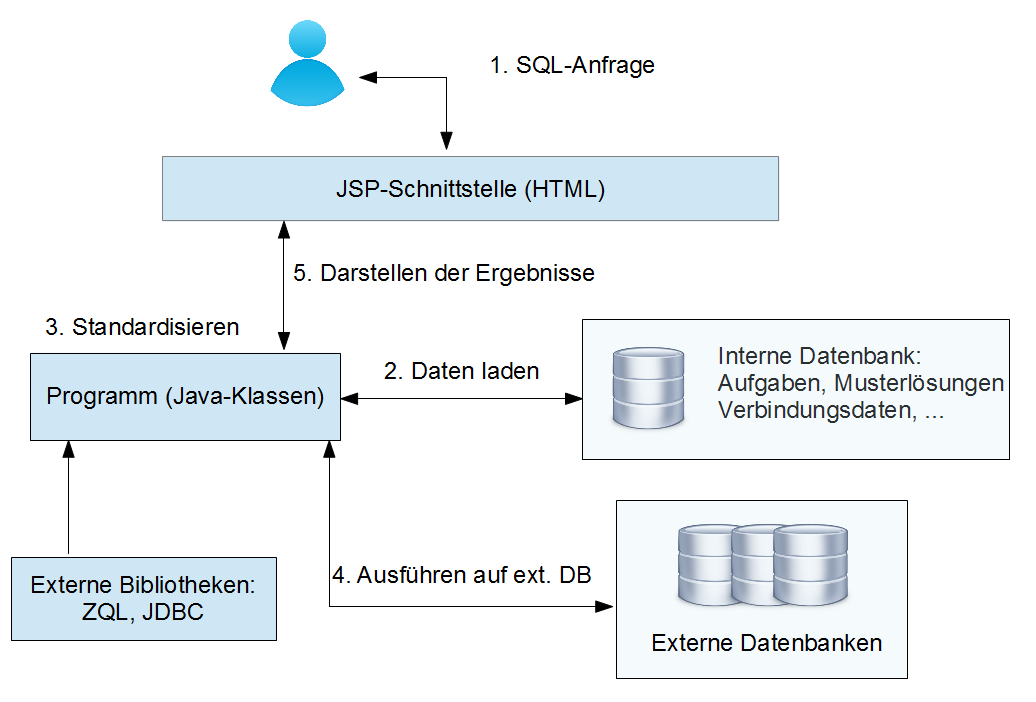
\includegraphics[scale=0.4]{schema.png}
\end{center}
\end{frame}

\begin{frame}[fragile]{Einschränkungen in der Praxis / Probleme}
\begin{itemize}
\item Nur Tabellen in \verb|FROM| zugelassen (keine Verbunde, Unterabfragen)
\item[$\to$] keine Implementierung von (bereits ausgearbeiteten) Verbundskonzepten
\item Parser versteht keine \verb|CREATE TABLE|-Anweisungen
\item[$\to$] Kenntnis über Spalten (Name, Datentyp, Eigenschaften) notwendig
\item[$\to$] rudimentäres Parsen von \verb|CREATE TABLE|-Anweisungen implementiert 
\item JDBC-Connector für DBMS zum Teil sehr unterschiedlich
\item[$\to$] Anbinden von neuen DBMS-Typen muss getestet werden
\end{itemize}

\end{frame}

\begin{frame}[fragile]{Fortsetzung}
\begin{itemize}
\item Erweitern des Parsers 
\item[$\to$] Umsetzen der Verbundskonzepte
\item Erkennen von unnötigem \verb|DISTINCT|
\item Ausweitung auf Behandlung aller SQL-Ausdrücke (\verb|UPDATE, DELETE|)
\item Ausarbeitung und Implementierung weiterer Konzepte (zB: unnötige Verbunde, ...)
\item transitiv-implizierte Formeln: \verb|a = b AND a = 5| $\to$ \verb|b = 5|
\item Beschränkung der Domänen: \verb|a > 2 AND a > 0| $\to$ \verb|a > 2|
%\item Ausbau der Webseite: Gruppierung von Aufgaben, Einfügen von Kategorien, ...
\end{itemize}
\end{frame}

%\begin{frame}[fragile]{Parser}
%\begin{itemize}
%\item Verwendung des Parsers ZQL (Open Source)
%\item einfach bedienbar und leicht erweiterbar
%\item Parser erzeugt Listen von \textit{Items} (\verb|SELECT, FROM, ORDER BY, GROUP BY|)
%\item und Parserbäume als (nicht binäre) Bäume (\verb|WHERE, HAVING|)
%\item arithmetische Ausdrücke als Binärbäume geparst
%\end{itemize}
%\end{frame}

%\begin{frame}[fragile]{Beispiel Parser (WHERE)}
%\begin{verbatim}
%SELECT * FROM test 
%WHERE a > 2 AND b = 3 AND c IS NULL
%\end{verbatim}
%\begin{center}
%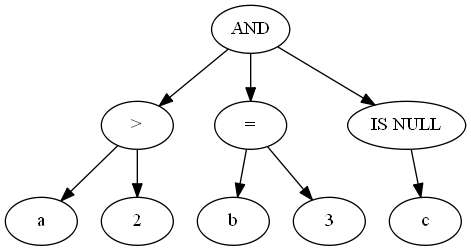
\includegraphics[scale=0.48]{bsp_parser.png}
%\end{center}
%\end{frame}


\section{Live Präsentation}

\end{document}


